\documentclass[11pt]{article}
\usepackage{geometry}                % See geometry.pdf to learn the layout options. There are lots.
\geometry{letterpaper}                   % ... or a4paper or a5paper or ... 
%\geometry{landscape}                % Activate for for rotated page geometry
%\usepackage[parfill]{parskip}    % Activate to begin paragraphs with an empty line rather than an indent
\usepackage{graphicx}
\usepackage{amssymb}
\usepackage{amsmath}
\usepackage{epstopdf}
\usepackage{hyperref}
\DeclareGraphicsRule{.tif}{png}{.png}{`convert #1 `dirname #1`/`basename #1 .tif`.png}



\graphicspath{
{/Users/Andy/Cruises_Research/ChiPod/Cham_Eq14_Compare/mfiles/Patches/}
}

\title{EQ14 - Computing gamma by patches}
\author{Andy Pickering}
%\date{}                                           % Activate to display a given date or no date



\begin{document}
\maketitle

\tableofcontents
\newpage


%~~~~~~~~~~~~~~~~~~~~~~~~~~~~~~
\section{Intro}

In this analysis i'm tyring to compute $\Gamma$ for EQ14 Chameleon data by patch instead of just at every point. The equation used is 

\begin{equation}
\Gamma=\frac{N^2 \chi}{2\epsilon <dT/dz>^2}
\end{equation}

Figure \ref{gam_cham} shows the distribution of estimated gammas using all the chamleon data, and using just the data between 60 and 180m depth. The median gamma from both is about 0.02, about ten times smaller than the usually assumed $\Gamma=0.2$.

\begin{figure}[htbp]
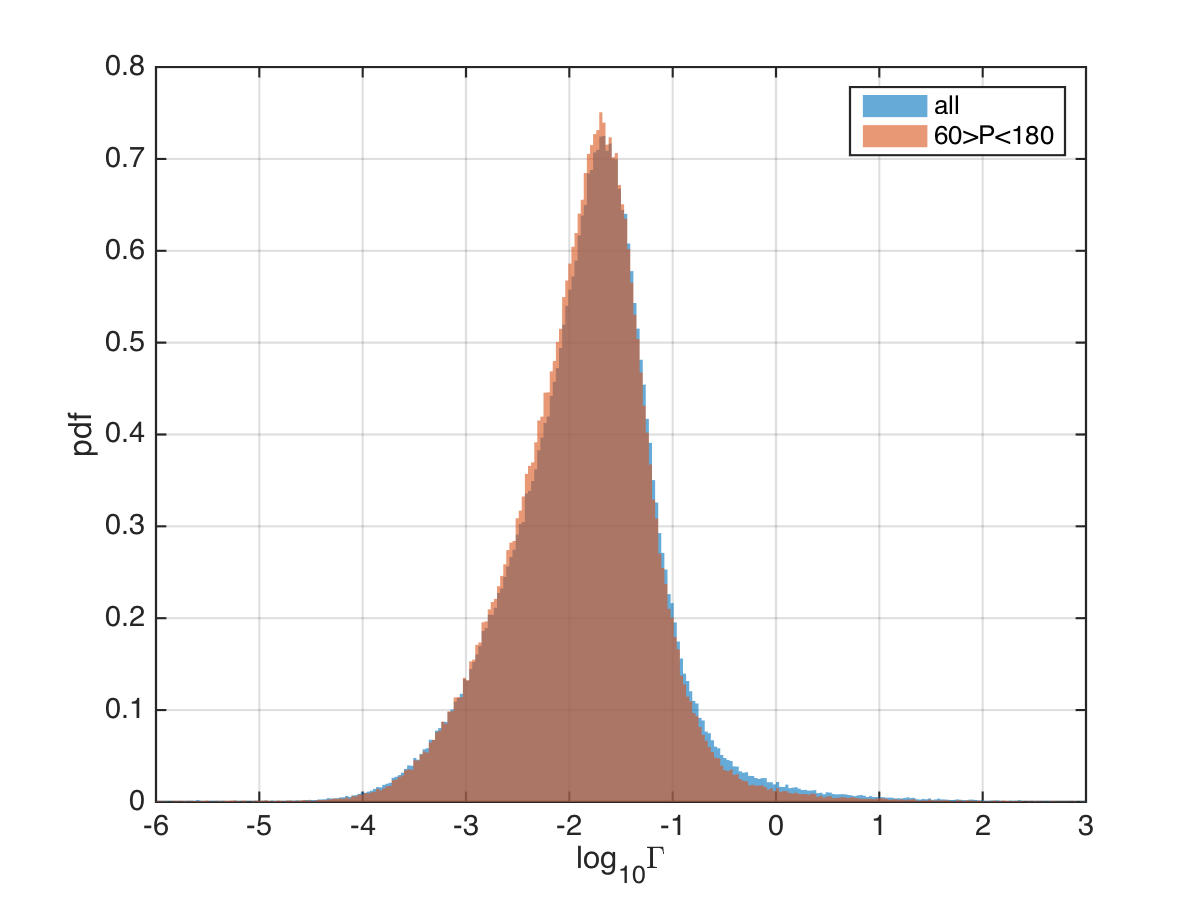
\includegraphics[scale=0.8]{gam_cham_hist.png}
\caption{Histogram of $\Gamma$ for all EQ14 chameleon profiles.}
\label{gam_cham}
\end{figure}


%~~~~~~~~~~~~~~~~~~~~~~~~~~~~~~
\section{Identifying Patches}

Code: \verb+Compute_gamma_by_patches.m+

I first identify patches (overturns) using potnential density computed from 1m binned temperature and salinity from Chameleon profiles.

\begin{itemize}
\item Figure \ref{psizebox} shows the distribution of patch sizes from all profiles (exluding those above 20m and below 180m). Only about 11\% of the orginal patches are in this good depth range. Most of the patches are very small (1-2m).
\item Figure \ref{epswot} shows $\epsilon$ with overturn locations plotted over. The majority of the identified overturns occur between 20-60m, associated with the diurnal cycle of turbulence. These probably shouldn't even be included in the chipod analysis since the assumed dynamics do not hold.
\item Below that, overturns generally co-occur with larger $\epsilon$ measured by chameleon shear probe. There are some that occur where chameleon $\epsilon$ is small, however.
\item Figure \ref{hists_allVspatch} shows distributions of all data versus just data within the identified patches. Patches are associated with lower N2 and dtdz, and higher epsilon. The distribution of chi does not appear to be significantly different.
\end{itemize}



\begin{figure}[htbp]
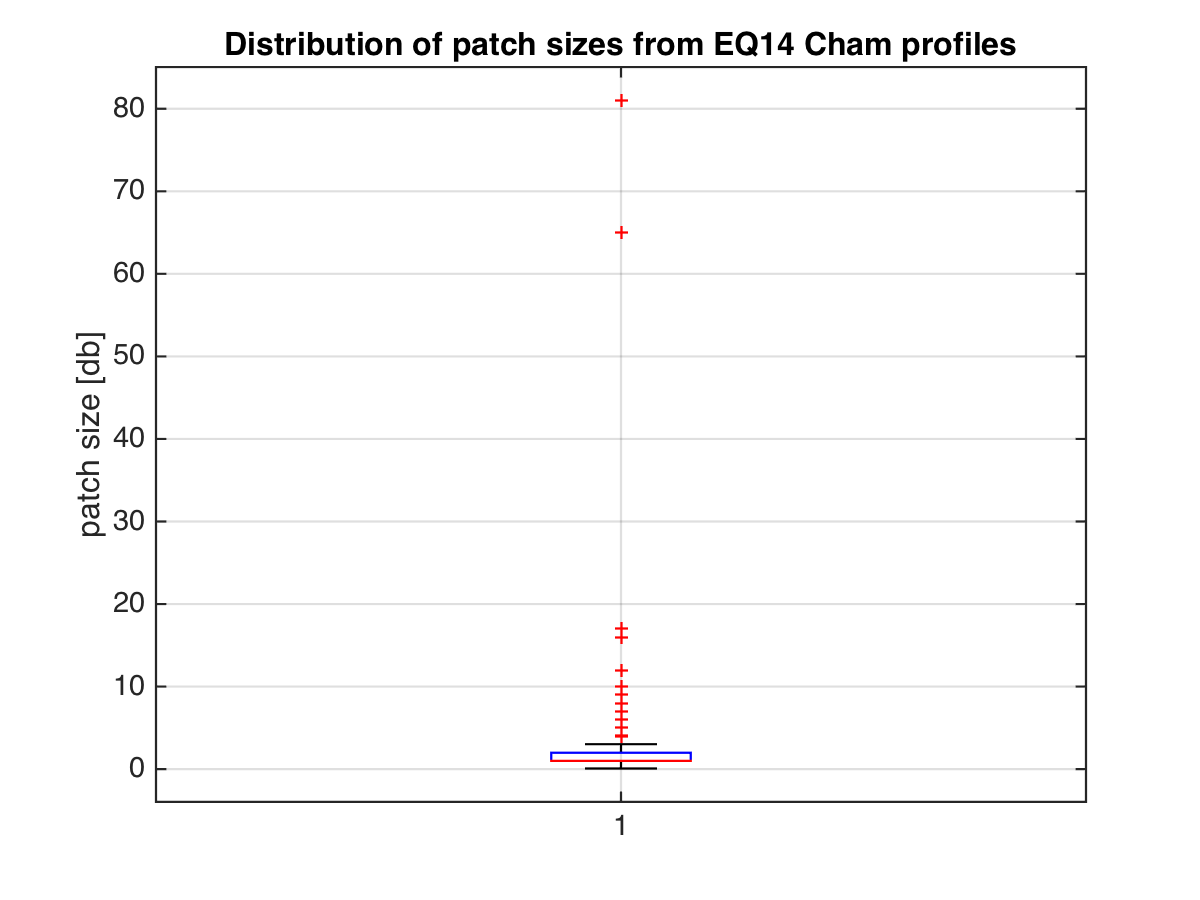
\includegraphics[scale=0.8]{GamByPatch_patchsize_boxplot.png}
\caption{Boxplot of the patch sizes for all EQ14 chameleon profiles. Only patches occuring at depths between 20 and 180 m are considered.}
\label{psizebox}
\end{figure}

\begin{figure}[htbp]
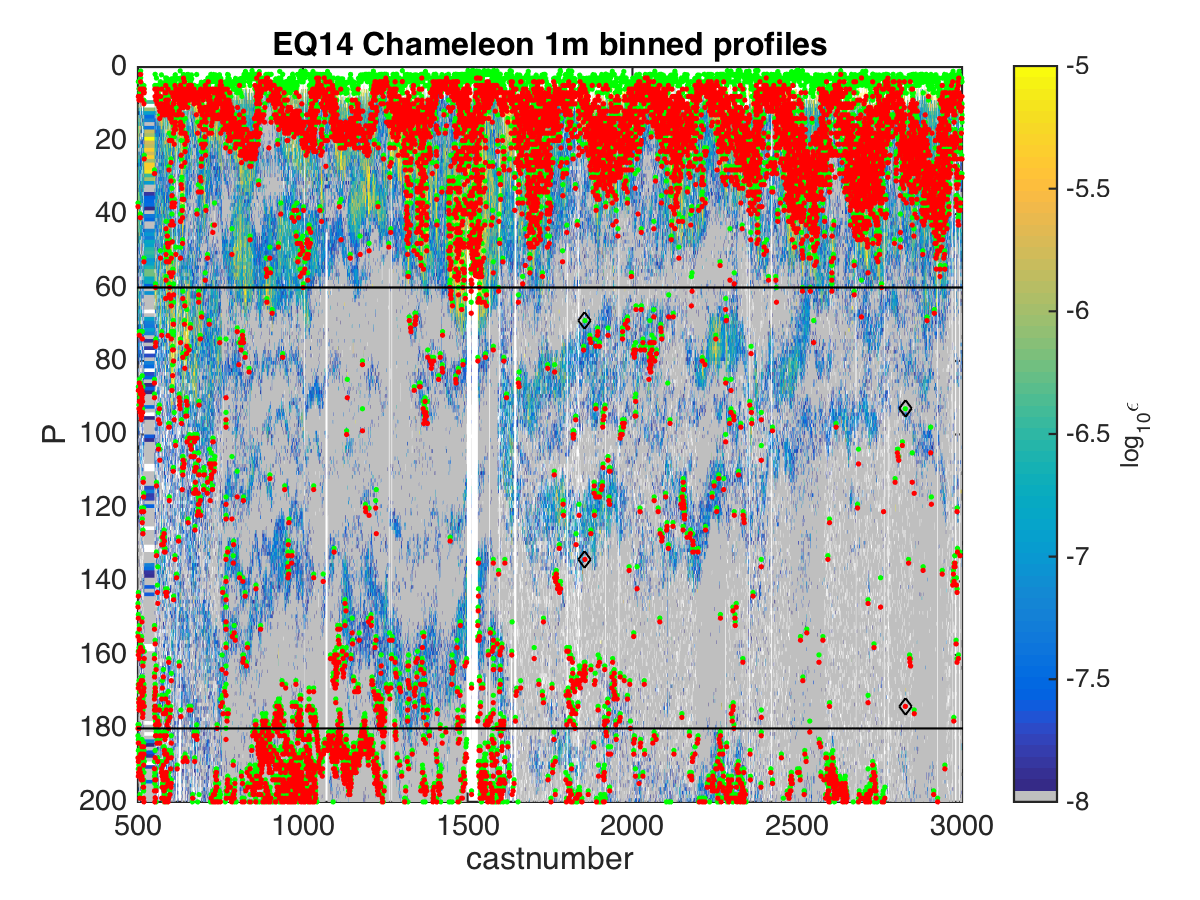
\includegraphics[scale=0.8]{GamByPatch_eps_pcolor_wpatches.png}
\caption{$\epsilon$ measured by chameleon shear probes on EQ14 profiles. Identified overturns are plotted in green/red. Black diamonds indicate overturns larger than 20m, these are ignored (there are only 2).}
\label{epswot}
\end{figure}


\begin{figure}[htbp]
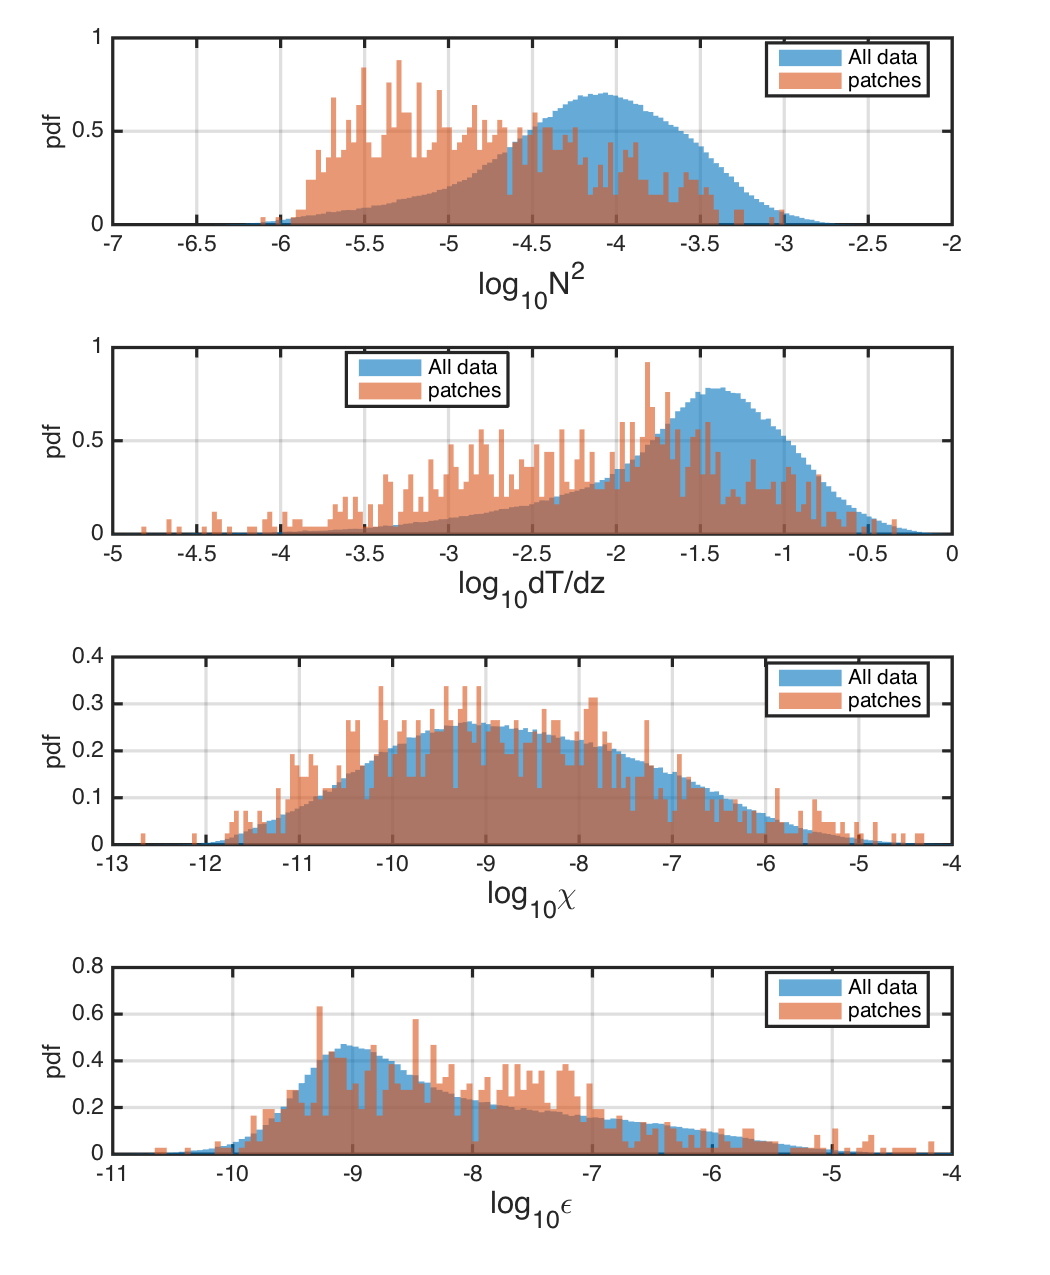
\includegraphics[scale=0.8]{hists_allVspatch.png}
\caption{Distributions of N2,dtdz,chi,eps from EQ14 chameleon profiles, for all data and just within patches.}
\label{hists_allVspatch}
\end{figure}


\clearpage
%~~~~~~~~~~~~~~~~~~~~~~~~~~~~~~
\section{Computing gamma by patch}

The next step is to compute $\Gamma$ over each patch. I will use $N^2$ and $dT/dz$ averaged over the patch (since most patches are very small, this probably won't differ too much?). For $\chi$ and $\epsilon$, I should compute these from spectra over the entire patch. This will involve hacking into the chameleon processing codes a bit... Before I do this, I will try just using the 1m binned values within each patch.

So far this doesn't seem to be giving me anything close to $\Gamma=0.2$ (figure \ref{hists_gamma_allVspatch}).

\begin{figure}[htbp]
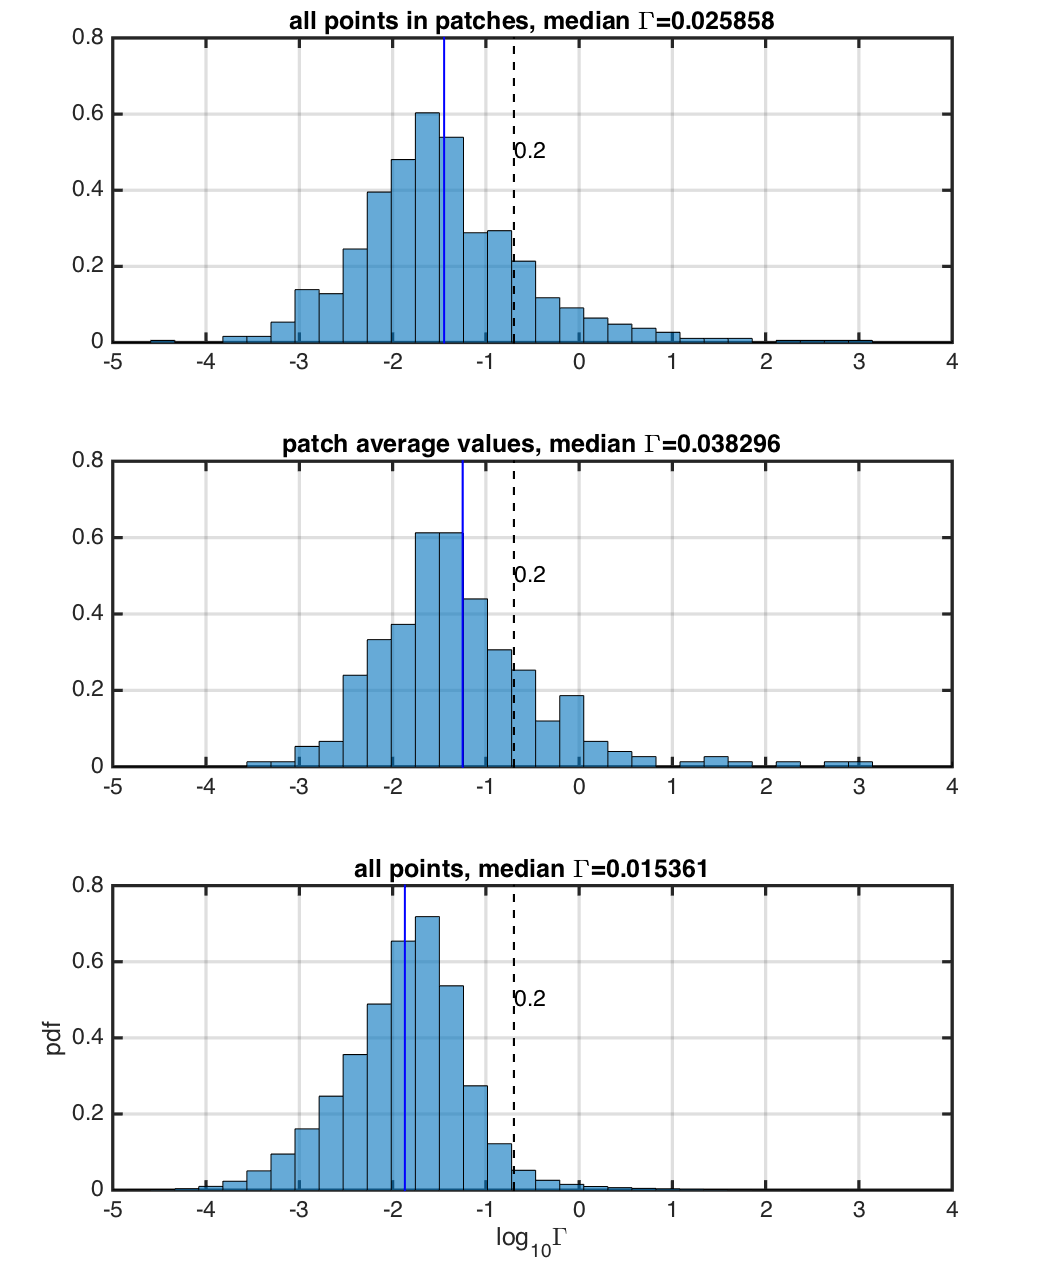
\includegraphics[scale=0.8]{hists_gamma_allVspatch.png}
\caption{Histograms of gamma for (1) all points within patches (2) using averaged values from patches (3) using all points. Only data between 60-180m depth is used for all. }
\label{hists_gamma_allVspatch}
\end{figure}



\end{document}  
